\usetikzlibrary{graphs,graphdrawing}
\usegdlibrary{trees}

\begin{frame}<1>[label=rbInsertCases]{red-black insert}
\begin{itemize}
\item default: insert as \nred{red} (no change to black node count), but\ldots
\item \myemph<2>{(1) if new node is root}: color \nblack{black}
\item \myemph<3>{(2) if parent is black}: keep child \nred{red}
\item \myemph<4>{(3) if parent and uncle is \nred{red}}: adjust several colors
\item \myemph<5>{(4) if parent is \nred{red}, uncle is \nblack{black}}, new node is right child
    \begin{itemize}
    \item perform a rotation, then go to case 5
    \end{itemize}
\item \myemph<6>{(5) if parent is \nred{red}, uncle is \nblack{black}}, new node is left child
    \begin{itemize}
    \item perform a rotation
    \end{itemize}
\end{itemize}
\begin{tikzpicture}[overlay, remember picture]
\coordinate (where) at ([yshift=1cm]current page.south);
\tikzset{
    box/.style={draw,very thick,fill=white,at=(where), anchor=south, align=left},
}
\begin{visibleenv}<2>
\node[box] {
    property: ``root is black'' \\
    no children $\rightarrow$ no worries about \# black nodes \\
    on different paths
};
\end{visibleenv}
\begin{visibleenv}<3>
\node[box] {
    property: ``children of \nred{red} node are \nblack{black}'' \\
    no change in \# of \nblack{black} nodes on paths 
};
\end{visibleenv}
\end{tikzpicture}
\end{frame}

\againframe<3>{rbInsertCases}

\againframe<4>{rbInsertCases}

\begin{frame}{case 3: parent, uncle are red}
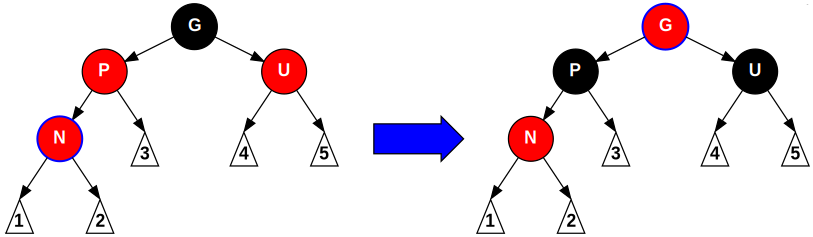
\includegraphics[width=0.9\textwidth]{Red-black_tree_insert_case_3}
\begin{itemize}
\item make grandparent \nred{red}, parent and uncle \nblack{black}
    \begin{itemize}
    \item (property: every path to leaf has same number of black nodes)
    \item just swapped grandparent and parent/uncle in those paths
    \end{itemize}
\item<2-> but\ldots what if grandparent's parent is red?
    \begin{itemize}
    \item (property: children of red node are black)
    \item solution: \myemph<3>{recurse to the grandparent}, as if it was just inserted
    \end{itemize}
\end{itemize}
    \imagecredit{image: Wikipedia/Abloomfi}
\end{frame}

\againframe<5>{rbInsertCases}

\begin{frame}{case 4: parent red, uncle black, right child}
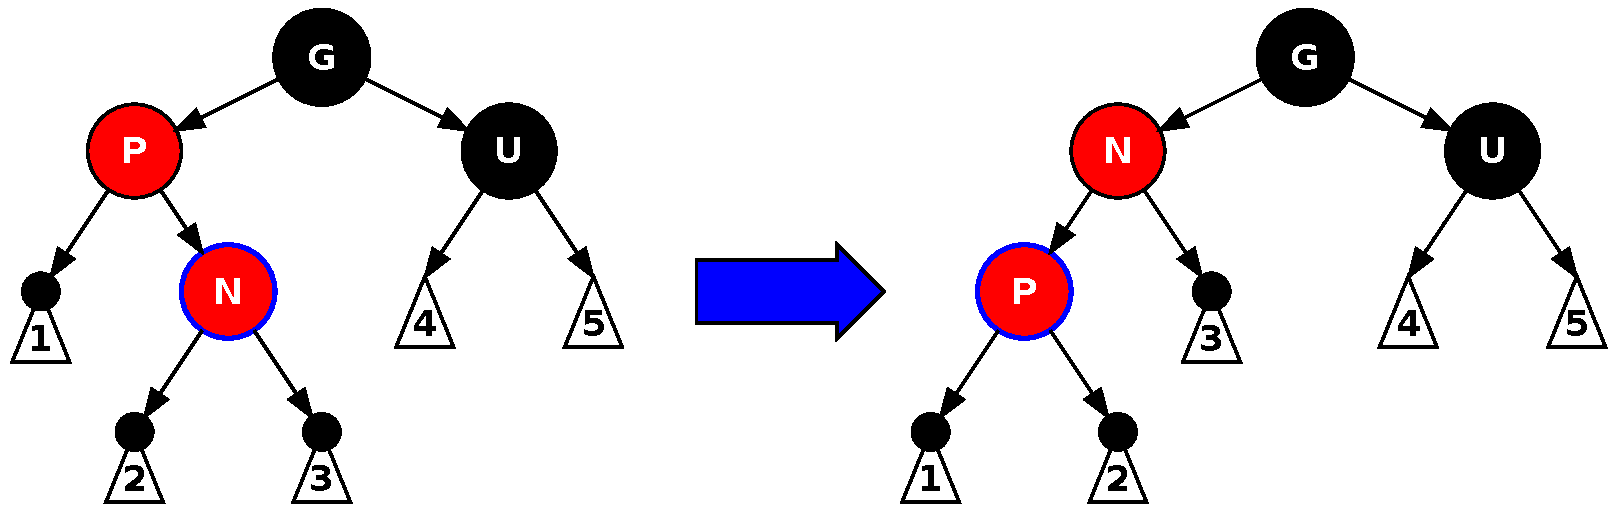
\includegraphics[width=0.9\textwidth]{Red-black_tree_insert_case_4}
\begin{itemize}
\item perform left rotation on parent subtree and new node
\item now case 5 (but new node is $P$, not $N$)
\end{itemize}
    \imagecredit{image: Wikipedia/Abloomfi}
\end{frame}

\againframe<6>{rbInsertCases}

\begin{frame}{case 5: parent red, uncle black, left child}
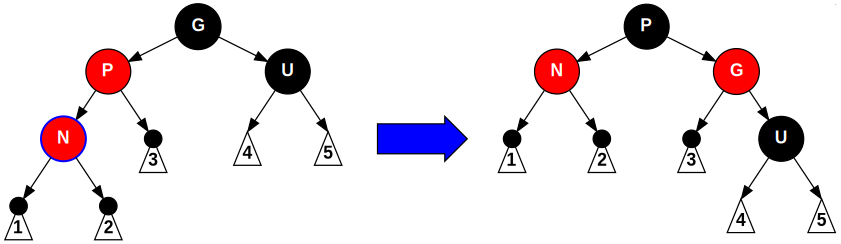
\includegraphics[width=0.9\textwidth]{Red-black_tree_insert_case_5}
\begin{itemize}
\item perform right rotation of grandparent and parent
\item swap colors of parent and grandparent
\item preserves properties:
\begin{itemize}
\item red parent's children are black
\item every path to leaf has same number of black nodes
\end{itemize}
\end{itemize}
    \imagecredit{image: Wikipedia/Abloomfi}
\end{frame}

\begin{frame}{example recursive case}
\begin{tikzpicture}
\tikzset{
    >=Latex,
    myt/.style={binary tree layout,level distance=2mm,sibling distance=25mm,nodes={draw,circle,very thick,inner sep=0.25mm,minimum width=1cm,align=center,font=\small,fill=white}},
    mytB/.style={myt,nodes={draw,circle,very thick,inner sep=0.25mm,minimum width=1cm,align=center,font=\small,fill=white}},
    R/.style={fill=red!20},
    B/.style={fill=black!90,text=white},
    null/.style={rectangle,draw=none,text=white,label={[font=\small]center:NULL}},
    inserted/.style={alt=<1-3>{draw=blue,ultra thick}},
    insertedB/.style={alt=<4-6>{draw=blue,ultra thick}},
    hiParUncle/.style={alt=<2-3>{draw=red,ultra thick,dashed}},
    hiParUncleB/.style={alt=<4-5>{draw=red,ultra thick,dashed}}
}
\begin{visibleenv}<1-4>
\begin{scope}[myt]
\graph {
    [fresh nodes,name=g] 100[B] -> {
        10[R,hiParUncleB] -> { 3[alt=<1-2>{B},alt=<3-4>{R},insertedB] -> {1[alt=<1-2>{R},alt=<3-4>{B},hiParUncle], 5[alt=<1-2>{R},alt=<3-4>{B},hiParUncle] ->[alt=<1>{white}] 8[second,inserted,R,alt=<1>{white}]}, 15[B] },
        200[B,hiParUncleB]
    }
};
\end{scope}
\end{visibleenv}
\begin{visibleenv}<5->
\begin{scope}[myt,sibling distance=15mm]
\graph {
    [fresh nodes,name=gB] 10[B] -> {
        3[R] -> {1[B], 5[B] -> 8[R,second]},
        100[R] -> {15[B], 200[B]}
    }
};
\end{scope}
\end{visibleenv}
\tikzset{
    box/.style={left=2cm of g 100,draw,thick,align=left},
}
\begin{visibleenv}<1>
    \node[box] {initially: \\
        leaves are \nblack{black} \checkmark \\
        \nred{red} node's children are \nblack{black} \checkmark \\
        same number of black nodes \\
        in every path from node to leaves \checkmark 
        };
\end{visibleenv}
\begin{visibleenv}<2>
    \node[box] {insert \textbf{\color{blue!70!black}8} \\
    initially make \nred{red} \\
    \myemph{case 3: parent, uncle are red}};
\end{visibleenv}
\begin{visibleenv}<3>
    \begin{scope}[mytB]
\graph {
    [fresh nodes,name=alt3] 3[B,desired at={([xshift=-6cm]g 3)}] -> { 1[R,hiParUncle], 5[R,hiParUncle] -> 8[R,second,inserted] }
};
    \end{scope}
    \node[above=0cm of alt3 3] {\textit{before:}};
    \draw[Latex-] (alt3 3.north east) -- ++(.5cm,.5cm);
    \node[box] {\myemph{case 3: parent, uncle are red}: \\
    grandparent becomes \nred{red} \\
    parent/uncle \nblack{black}
    };
\end{visibleenv}
\begin{visibleenv}<4>
    \node[box] {case 3 (parent, uncle are red) continued: \\
        recusively examine grandparent \textbf{\color{blue!70!black}3} \\
        \myemph{case 4: parent (of 3) is red} \\
        \hspace{1cm}\myemph{uncle is black, left child}
    };
\end{visibleenv}
\begin{visibleenv}<5>
    \begin{scope}[mytB]
\graph {
    [fresh nodes,name=alt5] 100[B,desired at={([xshift=-8cm,yshift=1cm]gB 10)}] -> {10[R] -> {3[R] -> {"\ldots"[draw=none],"\ldots"[draw=none]}, 15[B]},
        200[B]}
};
    \end{scope}
    \node[draw,thick,align=left,below=1cm of alt5 15] {\myemph{case 4: parent is red} \\
    \hspace{1cm}\myemph{uncle is black, left child}: \\
        perform right rotation \\ of parent + grandparent (of 3) \\
        (and swap parent/grandparent colors)
    };
    \draw[line width=.5mm,-Latex] ([xshift=1cm]alt5 200.east) -- ++(2cm,0cm);
\end{visibleenv}
\end{tikzpicture}
\end{frame}

